% ADD/REMOVE THE 'answers' OPTION TO INCLUDE/SUPPRESS SOLUTIONS
% \documentclass[11pt,addpoints]{exam}
\documentclass[11pt,addpoints,answers]{exam}

\newcommand{\hwnum}{2}
\newcommand{\duedate}{January 22}

% In order to compile this file you will need to get 'header.tex'
% and make the line below point to the appropriate file path
\RequirePackage{microtype}
\RequirePackage{mathtools}
\RequirePackage{amsthm}
\RequirePackage{amssymb}
\RequirePackage{xspace}
\RequirePackage[shortlabels]{enumitem}
\RequirePackage{xcolor}
\RequirePackage{hyperref}
\RequirePackage[capitalize,nameinlink,noabbrev]{cleveref} % must load after hyperref
\usepackage{fvextra} % To use Verbatim
\RequirePackage[boxed]{algorithm}
\RequirePackage[noend]{algpseudocode}
\RequirePackage{tikz}

\hypersetup{breaklinks=true,
    colorlinks=true,
    linkcolor=blue,
    filecolor=blue,
    citecolor=blue,
    urlcolor=blue}

\algrenewcommand{\algorithmiccomment}[1]{\texttt{//} #1}
\algrenewcommand\algorithmicrequire{\textbf{Input:}}
\algrenewcommand\algorithmicensure{\textbf{Output:}}


% allow cleveref to label and reference enumerables defined in the exam class.
% these automatically define corresponding \Crefname as well.

% https://tex.stackexchange.com/questions/126020/cleveref-doesnt-use-correct-capitalized-name-if-used-with-amsthm
\makeatletter
\if@cref@capitalise
\crefname{question}{Question}{Questions}
\Crefname{partno}{Part}{Parts}
\crefname{subpart}{Subpart}{Subparts)}
\crefname{subsubpart}{Subsubpart}{Subsubparts}
\else
\crefname{question}{question}{questions}
\crefname{partno}{part}{parts}
\crefname{subpart}{subpart}{subparts}
\crefname{subsubpart}{subsubpart}{subsubparts}
\fi
\makeatother

% numeric sets in "blackboard" font

\newcommand{\N}{\mathbb{N}}
\newcommand{\Z}{\mathbb{Z}}
\newcommand{\R}{\mathbb{R}}
\newcommand{\Q}{\mathbb{Q}}
\newcommand{\C}{\mathbb{C}}
\newcommand{\Prop}{\mathbb{P}}

% paired delimiters

\DeclarePairedDelimiter\abs{\lvert}{\rvert}
\DeclarePairedDelimiter\length{\lVert}{\rVert}
\DeclarePairedDelimiter\norm{\lVert}{\rVert}
\DeclarePairedDelimiter\parens{(}{)}
\DeclarePairedDelimiter\tuple{(}{)}
\DeclarePairedDelimiter\brackets{[}{]}
\DeclarePairedDelimiter\floor{\lfloor}{\rfloor}
\DeclarePairedDelimiter\ceil{\lceil}{\rceil}
\DeclarePairedDelimiter\round{\lfloor}{\rceil}
\DeclarePairedDelimiter\set{\{}{\}}
\DeclarePairedDelimiter\inner{\langle}{\rangle}

\newcommand{\bit}{\set{0,1}}

% asymptotics

\DeclareMathOperator{\Otil}{\tilde{O}}
\DeclareMathOperator{\poly}{poly}
\DeclareMathOperator{\polylog}{polylog}
\DeclareMathOperator{\negl}{negl}

% algorithms

\newcommand{\algo}[1]{\textsc{#1}}

\newcommand{\memo}{\text{memo}}
\newcommand{\tabl}{\text{table}}
\newcommand{\backtrack}{\text{backtrack}}

\newcommand{\ALG}{\text{ALG}}
\newcommand{\OPT}{\text{OPT}}
\newcommand{\weight}{\text{weight}}
\newcommand{\val}{\text{value}}

% computability

% named language
\newcommand{\lang}[1]{L_{\text{#1}}}
% computational problem
\newcommand{\cproblem}[1]{\ensuremath{\text{#1}}\xspace}
% class of languages
\newcommand{\class}[1]{\ensuremath{\mathsf{#1}}\xspace}

\newcommand{\qst}{q_{\text{start}}}
\newcommand{\qacc}{q_{\text{acc}}}
\newcommand{\qrej}{q_{\text{rej}}}

\newcommand{\Lbarber}{\lang{BARBER}}
\newcommand{\atm}{\lang{ACC}}
\newcommand{\htm}{\lang{HALT}}
\newcommand{\ehtm}{\lang{$\varepsilon$-HALT}}
\newcommand{\eqtm}{\lang{EQ}}
\newcommand{\etm}{\lang{$\emptyset$}}
\newcommand{\epstm}{\lang{$\set{\varepsilon}$}}
\newcommand{\Lprop}{\lang{$\Prop$}}
\newcommand{\LSigmastar}{\lang{$\Sigma^*$}}

% complexity

\newcommand{\yes}{\ensuremath{\text{YES}}}
\newcommand{\no}{\ensuremath{\text{NO}}}

\newcommand{\DTIME}{\class{DTIME}}
\renewcommand{\P}{\class{P}}
\newcommand{\NP}{\class{NP}}
\newcommand{\NPH}{\class{NPH}}
\newcommand{\NPC}{\class{NPC}}
\newcommand{\coNP}{\class{coNP}}

\newcommand{\MAZE}{\cproblem{MAZE}}
\newcommand{\PALINDROME}{\cproblem{PALINDROME}}
\newcommand{\TSP}{\cproblem{TSP}}
\newcommand{\SAT}{\cproblem{SAT}}
\newcommand{\CSAT}{\cproblem{CSAT}}
\newcommand{\TSAT}{\cproblem{3SAT}}
\newcommand{\VC}{\cproblem{VERTEX-COVER}}
\newcommand{\SC}{\cproblem{SET-COVER}}
\newcommand{\HC}{\cproblem{HAMCYCLE}}
\newcommand{\HP}{\cproblem{HAMPATH}}
\newcommand{\IS}{\cproblem{IS}}
\newcommand{\CLIQUE}{\cproblem{CLIQUE}}
\newcommand{\SSUM}{\cproblem{SUBSET-SUM}}
\newcommand{\KNAPSACK}{\cproblem{KNAPSACK}}
\newcommand{\MAXCUT}{\cproblem{MAX-CUT}}

% randomness

\DeclareMathOperator*{\Var}{Var}
\DeclareMathOperator*{\Ex}{\mathbb{E}}

\newcommand{\RP}{\class{RP}}
\newcommand{\coRP}{\class{coRP}}
\newcommand{\BPP}{\class{BPP}}
\newcommand{\ZPP}{\class{ZPP}}
\newcommand{\BQP}{\class{BQP}}

%%% misc

\newcommand{\eps}{\varepsilon}

%%% theorems

\theoremstyle{plain}            % following are "theorem" style

\newtheorem{theorem}{Theorem}
\newtheorem{lemma}[theorem]{Lemma}
\newtheorem{corollary}[theorem]{Corollary}
\newtheorem{proposition}[theorem]{Proposition}
\newtheorem{claim}[theorem]{Claim}
\newtheorem{fact}[theorem]{Fact}
\newtheorem{openproblem}[theorem]{Open Problem}

\theoremstyle{definition}       % following are def style

\newtheorem{definition}[theorem]{Definition}
\newtheorem{conjecture}[theorem]{Conjecture}
\newtheorem{protocol}[theorem]{Protocol}
\newtheorem{exercise}[theorem]{Exercise}

\theoremstyle{remark}           % following are remark style

\newtheorem{example}[theorem]{Example}
\newtheorem{remark}[theorem]{Remark}
\newtheorem{note}[theorem]{Note}

%%% for homework and section notes

\newcommand{\commonheader}[2]{
    \pagestyle{headandfoot}
    \setlength{\headheight}{26pt}
    \setlength{\headsep}{16pt}

    \header
        {\small{\textbf{EECS 376: Foundations of Computer Science}} \\ \footnotesize{\textbf{University of Michigan, Winter 2025}}}
        {#1}
        {#2}

    \firstpageheadrule
    \runningheadrule

    \footer
        {}
        {\thepage}
        {}
}

\newcommand{\hwheader}{
    \commonheader
        {\Large \textbf{Homework \hwnum}}
        {\small \textbf{Due 8:00pm, \duedate\\ {\tiny(accepted until 9:59 pm, no credit after)}}}
}

\newcommand{\hwslnheader}{
    \commonheader
    	{}
        {\Large \textbf{Solutions to Homework \hwnum}}
    \printanswers
}

\newcommand{\notesheader}{
    \commonheader
    	{}
        {\Large \textbf{Discussion Notes \sectionnum}}
}

\newcommand{\practiceheader}{
    \commonheader
    	{}
        {\Large \textbf{Discussion Worksheet \sectionnum}}
}

\newcommand{\practiceslnheader}{
    \commonheader
    	{}
        {\Large \textbf{Solutions to Discussion Worksheet \sectionnum}}
}

\newcommand{\reviewheader}{
    \commonheader 
    \smallskip
    	{}
        {\Large \textbf{Midterm Review Notes}}
}

\newcommand{\hwpreface}{

\noindent This homework has \numquestions\ questions, for a total of \numpoints\ points and \numbonuspoints\ extra-credit points.

\noindent Unless otherwise stated, each question requires \emph{clear}, \emph{logically correct}, and \emph{sufficient} justification to convince the reader.

\noindent For bonus/extra-credit questions, we will provide very limited guidance in office hours and on Piazza, and we do not guarantee anything about the difficulty of these questions.
 
\noindent We strongly encourage you to typeset your solutions in \LaTeX.

\noindent If you collaborated with someone, you must state their name(s). You must \emph{write your own solution} for all problems and \emph{may not use any other student’s write-up}.
}

\newcommand{\hint}[1]{
\emph{Hint}: #1
}

% exam class setup
\pointsinmargin
\pointpoints{pt}{pts}
\bonuspointpoints{EC pt}{EC pts}
\marginpointname{ \points}
\marginbonuspointname{ \bonuspoints}


\ifprintanswers
\hwslnheader   % header for solutions
\else
\hwheader   % header for homework
\fi

\begin{document}

\hwpreface

\begin{questions}

  \addtocounter{question}{-1}
  \question[0] \textbf{Before you start; before you submit.} \nopagebreak
  
  \begin{parts}
    \part Before starting this assignment, carefully read \href{https://drive.google.com/file/d/1QidTYWPi4SeJLjT5I1MkhsQJvAnk6noY/view?usp=drive_link}{Handout 3} about ``giving an algorithm,'' and follow it in your solutions.

    \part Correctness arguments and runtime analysis for divide-and-conquer/recursive algorithms should follow the recommended structure described in this week's discussion worksheet.

    \part If applicable, state the name(s) and uniqname(s) of your collaborator(s).

    \begin{solution}
       
    \end{solution}

  \end{parts}

  \question[10] \textbf{Self assessment.} \nopagebreak
  
  Carefully read and understand the posted solutions to the previous homework.
  Identify one part for which your own solution has the most room for improvement (e.g., has unsound reasoning, doesn’t show what was required, could be significantly clearer or better organized, etc.).
  Copy or screenshot this solution, then in a few sentences, explain what was deficient and how it could be fixed.

  (Alternatively, if you think one of your solutions is significantly \emph{better} than the posted one, copy it here and explain why you think it is better.)

  If you didn't do last week's homework, choose a problem from it that looks challenging to you, and in a few sentences, explain the key ideas behind its solution in your own words.

  \begin{solution}
  
        % Easter egg for those using LaTeX!
        % Here's how you can insert an image in LaTeX, in case you need to include a screenshot
        % 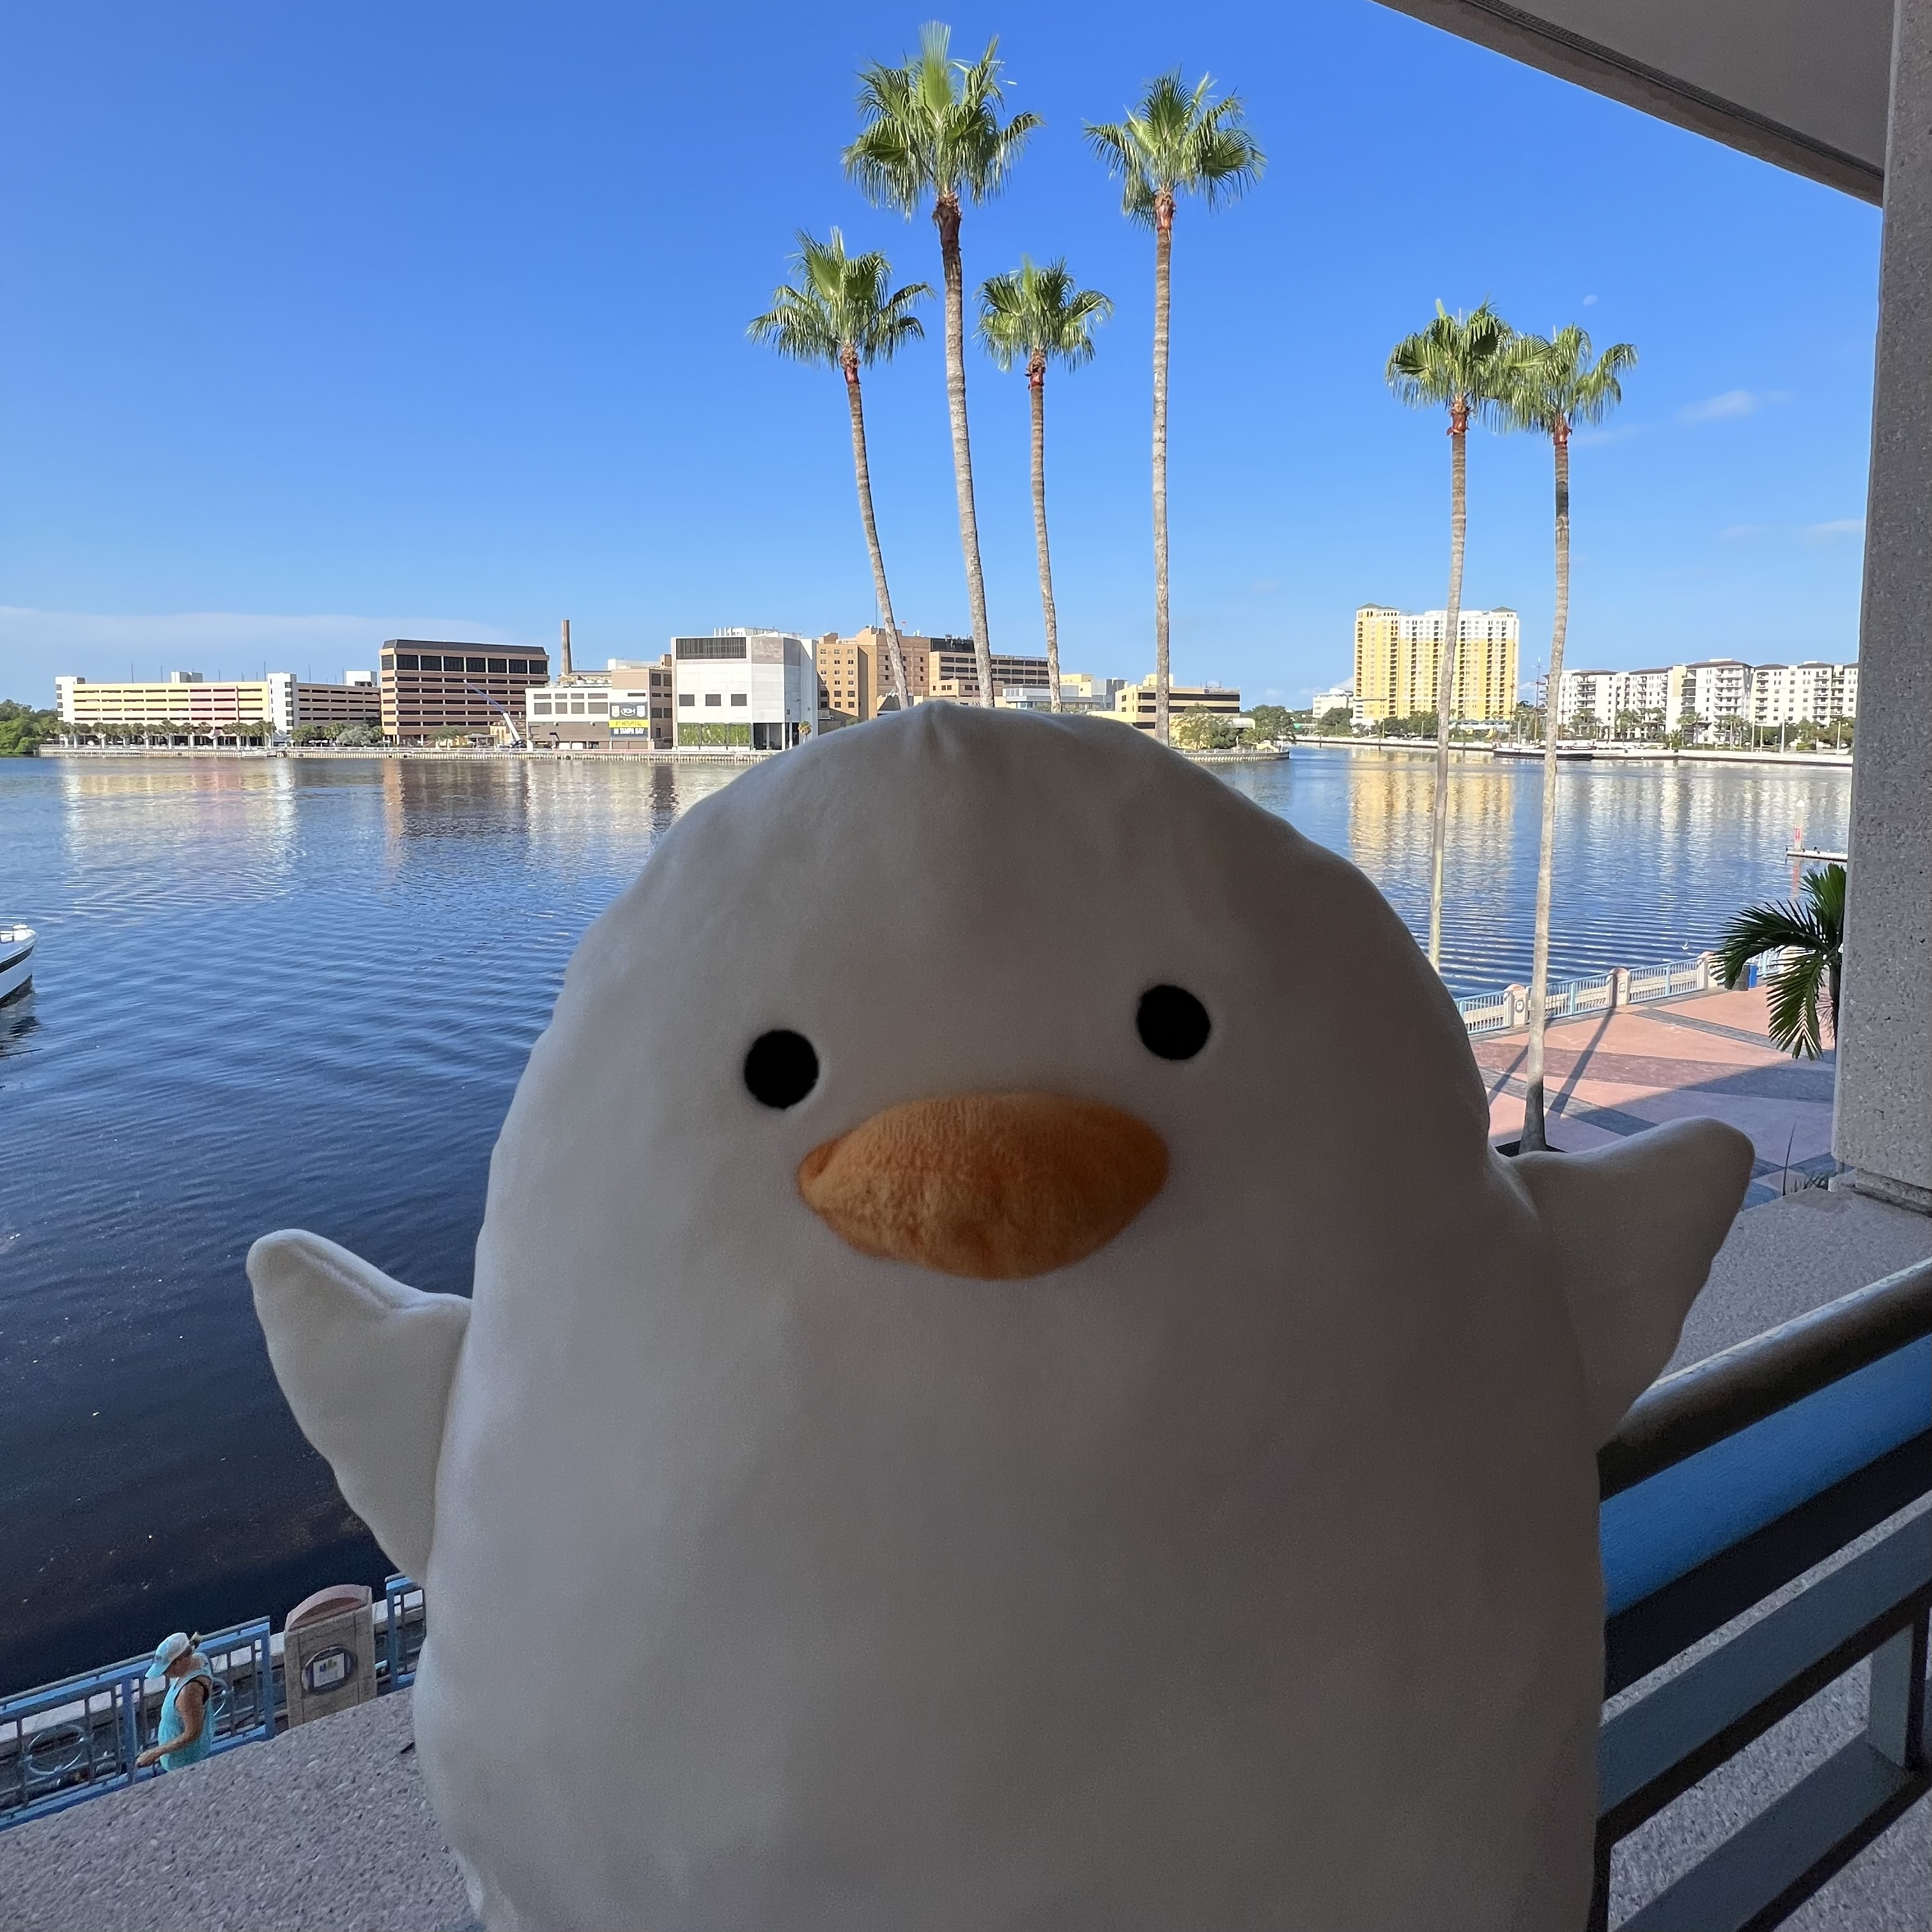
\includegraphics[width=0.5\linewidth]{waquackquack.jpg} % Adjust the dimension as you need
        
  \end{solution}


  \question \textbf{(Potential) infinite games.} \label{potential-infinite-games}

  Recall that the potential method requires several properties to hold in order to prove that a given process must eventually halt, within a certain number of ``time units.''
  These requirements include (but are not limited to):
  \begin{enumerate}[itemsep=0pt]
  \item the potential cannot go below some fixed lower bound; or if it does, the process must immediately halt.\footnote{In class we required a lower bound of zero, which is without loss of generality, but a fixed lower bound suffices.}\label{lower-bound}
  
  \item the potential must \emph{decrease by (at least) some fixed positive amount} with each time unit.\label{decrease}
  \end{enumerate}

  For each of the following processes and candidate potential functions, state with justification whether they satisfy both of the above properties.
  If not, either describe an alternative potential function that does satisfy both properties (and allows us to conclude that the process must halt), or briefly explain why the process might not ever halt (and hence there is \emph{no} valid potential function for the process).

  \begin{parts}

\part[8] Consider a one-player game involving a pile of maize and blue chips.
  Initially, there is a finite number of each color of chip.
  The player repeatedly takes a ``turn'' until no chips remain in the pile, if this ever happens. In each turn, the player must \emph{remove} one chip of its choice from the pile, and if the removed chip is maize, the player may \emph{add} up to \emph{three blue chips} to the pile.

  Define a time unit to be a round of the game, and the potential~$n_{i}$ after~$i$ rounds to be the total number of chips in the pile. The game ends when there is no remaining chips in the pile, i.e., $n_i = 0$.

    \begin{solution}
    
    \end{solution}

    \part[8] Eric is playing a chasing game with his naughty duck Waquackquack. Initially, Waquackquack is $d > 0$ miles ahead of Eric. On each ``turn", Waquackquack waddles forward by a fixed distance of 1 mile, then Eric runs \emph{half} the remaining distance to Waquackquack. The game ends when Eric catches Waquackquack, if this ever happens. 

    Define a time unit to be one turn of this chase, and let the potential~$d_i$ after $i$ turns to be the remaining distance between Eric and Waquackquack. The chase ends when Eric catches Waquackquack, i.e., when $d_i = 0$. 

    \begin{solution} 
    
    \end{solution}

  \end{parts}
  

\question \textbf{Potential functions of functions.}

For each of the following functions, determine whether the function \emph{must} eventually halt, regardless of the input. 

If your answer is `yes', prove it by defining and analyzing a potential function in terms of the variable(s) in the algorithm. Otherwise, give a specific input that causes the function to loop along with a brief explanation for why it loops on that input. 

\emph{Reminder:} When defining a potential function, you need to also define the ``time unit" in a way that your potential function meets the two requirements outlined in \cref{potential-infinite-games}.
    
    \begin{parts}

    \part[6] \begin{minipage}{\linewidth}
    \begin{algorithm}[H]
        \begin{algorithmic}[1]
        \Require{positive integers $a$ and $b$}
        \Function{Func}{$a$, $b$}
            \If{$a=1$ \textbf{or} $b=1$ \textbf{or} $a=b$} 
                \State \Return $0$ 
            \EndIf
            \If{$a>b$} 
                \State \Return \Call{Func}{$a/2, 2b$} 
            \Else
                \State \Return \Call{Func}{$2a, b/2$} 
            \EndIf
        \EndFunction
        \end{algorithmic}
    \end{algorithm}
    \end{minipage}

    \begin{solution} 

    \end{solution}

    \part[8] \begin{minipage}{\linewidth}
    \begin{algorithm}[H]
        \begin{algorithmic}[1]
        \Require{positive integers $a$ and $b$}
        \Function{Alg}{$a$,$b$}
            \If{$a \leq b$} 
                \State \Return $b$ 
            \EndIf
            \If{$b$ is even} 
                \State \Return \Call{Alg}{$a-1, b+1$} 
            \Else
                \State \Return \Call{Alg}{$a, b+1$} 
            \EndIf
        \EndFunction
        \end{algorithmic}
    \end{algorithm}
    \end{minipage}

    \begin{solution}
      
    \end{solution}

    \part [8]
    \begin{minipage}{\linewidth}
    \begin{algorithm}[H]
    \begin{algorithmic}[1]
    \Require{a positive integer $x$}
    \Function{Foo}{$x$}
        \While{$x > 10$}
            \If{$x$ is odd}
                \State{$x \gets x + 3$}
            \Else
                \State{$x \gets x/2$}
            \EndIf
        \EndWhile
    \EndFunction
    \end{algorithmic}    
    \end{algorithm}
    \end{minipage}

    \begin{solution}

    \end{solution}

\end{parts}

    \question \textbf{Can you \emph{master} the sorting algorithms?}
    
    In this problem, we will analyze the runtime recurrence of two sorting algorithms (which are both correct!), namely,  \textsc{SlowSort} and \textsc{StoogeSort}. For each of the following algorithms,
    \begin{enumerate}
        \item give (with brief justification\footnote{You may refer to specific lines in the algorithm.}) a recurrence for the algorithm's running time $T(n)$ as a function of the input array size~$n$, and
        \item state whether the Master Theorem is applicable to the recurrence, and if so, use it to give the closed-form solution; if not, explain why not. 
    \end{enumerate}

  \begin{parts}

  \part [6]
        \begin{minipage}{\linewidth}
        \begin{algorithm}[H]
          \begin{algorithmic}[1]
            \Function{SlowSort}{$A[1, \ldots, n]$}
              \State \Call{SlowSort}{$A [1, \ldots, \floor{\frac{n}{2}}]$}
              \State \Call{SlowSort}{$A[\floor{\frac{n}{2}}+1, \ldots, n]$}
              \If{$A [\floor{\frac{n}{2}}] > A [n]$}
                \State swap $A[\floor{\frac{n}{2}}]$ and $A[n]$
              \EndIf
              \State \textsc{SlowSort}$( A [ 1, \ldots, n-1 ])$ 
              \State \Return $A$
            \EndFunction
          \end{algorithmic}
        \end{algorithm}
      \end{minipage}

  \begin{solution}

  \end{solution}

    \part[6]
    \begin{minipage}{\linewidth}
      \begin{algorithm}[H]
        \begin{algorithmic}[1]
          \Function{StoogeSort}{$A[1, \ldots, n]$}
          \If{$n=1$}
            \State \Return $A$
          \EndIf
          \If{$n=2$ \textbf{and} $A[1] > A[n]$}
            \State swap $A[1]$ and $A[n]$
          \EndIf
          \If{$n > 2$}
            \State $t \gets \lceil 2n/3 \rceil$
            \State \Call{StoogeSort}{$A[1, \ldots, t]$}
            \State \Call{StoogeSort}{$A[n-t+1, \ldots, n]$}
             \State \Call{StoogeSort}{$A[1, \ldots, t]$}
          \EndIf
          \State \Return $A$
          \EndFunction
        \end{algorithmic}
      \end{algorithm}
    \end{minipage}
    
    \begin{solution}

    \end{solution}
 
  \end{parts}

  \question \textbf{Karatsuba for polynomials.} 

  \emph{If you haven't already, carefully read \href{https://drive.google.com/file/d/1QidTYWPi4SeJLjT5I1MkhsQJvAnk6noY/view?usp=drive_link}{Handout 3} about ``giving an algorithm,'' and follow it for the next two problems.}

  In lecture, we have seen how the Karatsuba algorithm reduces the number of multiplications needed for mutiplying large integers. In this problem, we will see how a similar idea can be used to multiply polynomials efficiently. 

  Let $A(x) = a_0 + a_1 x + \ldots a_{n-1} x^{n-1}$ and $B(x) = b_0 + b_1 x + \ldots + b_{n-1} x^{n-1}$ be two polynomials of degree\footnote{The degree of a polynomial is the highest power of the variable (like $x$) in the polynomial when it is written in its standard form.} at most $n-1$. For simplicity, assume that $n$ is a power of 2, and that arithmetic operations (e.g., addition, multiplication) between two coefficients can be done in constant time. 

  As an example, the product of two polynomials of degree 1, $A(x) = 1 + 2x$ and $B(x) = 3 + 4x$ is 
  \[
    A(x) \cdot B(x) = (1 + 2x)(3 + 4x) = 3 + 10x + 8x^2 \text .
  \]

  We can use a divide-and-conquer approach to compute the coefficients of the product polynomial $A(x) \cdot B(x)$ in $O(n^{\log_2 3})$ time. To do this, we first split the polynomials into their higher-degree and lower-degree terms
  \begin{align*}
    A(x) &= p(x)\cdot x^{n/2} + q(x)\\
    B(x) &= r(x)\cdot x^{n/2} + s(x)
\end{align*}

    where $p(x)$ represents the higher-degree $n/2$ terms of $A(x)$ (with the $x^{n/2}$ factored out) and $q(x)$ represents the lower-degree $n/2$ terms; and similarly with $r(x)$ and $s(x)$ for $B(x)$. 

    \begin{parts}
        \part [4] \label{karatsuba-a} Show that 
        \[
            A(x) \cdot B(x) = (p(x)\cdot r(x))\cdot x^n + (p(x)\cdot s(x) + q(x)\cdot r(x))\cdot x^{n/2} + (q(x)\cdot s(x)) \text .
        \]

        \begin{solution}

        \end{solution}

        \part [4] Show that the middle term in \cref{karatsuba-a}, $p(x)\cdot s(x) + q(x)\cdot r(x)$, can be computed using only one multiplication of polynomials. 

        \begin{solution}

        \end{solution}

        \part [10] Give an $O(n^{\log_2 3})$-time divide-and-conquer algorithm to compute the coefficients of the product polynomial $A(x) \cdot B(x)$. Remember to include correctness proof and runtime analysis in your solution. 
        \begin{solution}

 
        \end{solution}
    \end{parts}

\question \textbf{Sorting out errors.} \nopagebreak

  A coding project requires $n$ different software modules, each with a unique loading priority. Modules must be loaded in an order that respects their priorities---modules with lower priority values (indicating higher precedence) should be loaded before those with higher priority values. If a module with a higher priority value (lower precedence) is loaded before one with a lower priority value, an error message is output for each such conflict.

  For example, given the following load order (where the modules are loaded from left to right and are represented and referred to by their priority values):

  \[[4,2,3,1]\]

  There are 5 error messages output:
  \begin{itemize}
    \item Module 1 causes 3 error messages, as Modules 4, 2, and 3 are all loaded before it.
    \item Module 2 causes 1 error message, as Module 4 is loaded before it.
    \item Module 3 causes 1 error message, as Module 4 is loaded before it.
    \end{itemize}

  In this problem we are concerned with algorithm that determine the number of error messages that will be output.
  The input is an array $A[1,\ldots,n]$ of the modules' load priorities, from the beginning of the load order to the end.
  (So, $A[1]$ is the priority of the first module being loaded, and $A[n]$ is the priority of the last module.)
  The desired output is the total number of error messages.
  (Throughout this question, assume that any two priorities can be looked up and compared in constant time, independent of~$n$.)

  \begin{parts}
    \part[4] Describe briefly, clearly, and precisely (in English) a simple brute-force algorithm for this problem; do not give pseudocode.
    State, with brief justification, a $\Theta(\cdot)$ bound on its (worst-case) running time as a function of~$n$.
    You do not need to give a formal proof.

    \begin{solution}

    \end{solution}

    \part[10]
    Suppose that both the front half and back half of the load order (i.e., the two halves of the array~$A$) happen to be sorted in proper order of priorities, though the entire line may not be. \label{sort-error-b}

    Give an $O(n)$-time algorithm that outputs the number of error messages in this scenario.
    Your description of the algorithm can be in English or in pseudocode (as you prefer), but it should be clear and precise.

    \hint{This is the same setup as for the \textsc{Merge} subroutine (from \textsc{MergeSort} algorithm), but a different task.}
    
    \begin{solution}

    \end{solution}

    \part[8] Give an $O(n \log n)$-time divide-and-conquer algorithm for the error message counting problem.

    \hint{Modify the \textsc{MergeSort} algorithm slightly, to both sort \emph{and} count. You may call your algorithm in \cref{sort-error-b} as subroutine.}
    
    \begin{solution}

    \end{solution}

  \end{parts}

\ifprintanswers
\else
\newpage
\fi

    \bonusquestion \textbf{Graphs have potential too, maybe (optional extra credit).} 

    \emph{Reminder: For bonus/extra-credit questions, we will provide very limited guidance in office hours and on Piazza, and we do not guarantee anything about the difficulty of these questions.}
   
    Recall that a \emph{connected graph} is a graph in which there is a path between every pair of vertices. The following algorithm determines (or attempts to determine) a certain property of a connected graph. 
    
    \begin{minipage}[t]{\linewidth}
    \begin{algorithm}[H]
      \begin{algorithmic}[1]
        \Require{a connected graph $G$}
        \Ensure{[\textbf{FOR YOU TO DETERMINE}: truth value indicating some property of $G$]}
        \Function{Algorithm}{$G$}
            \State Initialize empty sets $S$, $A$, and $B$
            \State $v \gets$ vertex in $G$ with the lowest \href{https://en.wikipedia.org/wiki/Lexicographic_order}{lexicographic} order
            \State $S \gets S \cup \set{v}$ \Comment{Add $v$ to set $S$}
            \State $A \gets A \cup \set{v}$  \Comment{Add $v$ to set $A$}
            \While{$S$ is not empty}
                \State $u \gets $ vertex in $S$ with the lowest lexicographic order
                \State Remove $u$ from $S$
                \For {each neighbor $t$ of $u$}
                    \If{$t$ and $u$ are both in $A$ \textbf{or} both in $B$}
                        \State \Return{False}
                    \EndIf
                    \If{if $t$ is in neither $A$ nor $B$}
                        \State $S \gets S \cup \set{t}$ \Comment{Add $t$ to set $S$}
                        \State{Add $t$ to a different set from $u$ ($A$ or $B$)}
                    \EndIf
                \EndFor
            \EndWhile
            \State \Return{True}
        \EndFunction
      \end{algorithmic}
    \end{algorithm}
  \end{minipage}

  \begin{parts}

  \bonuspart [3] Determine whether \textsc{Algorithm} \emph{must} eventually terminate, regardless of the input. If your answer is `yes', prove it by defining and analyzing a potential function. Otherwise, give a specific graph that causes the function to loop along with a brief explanation for why it loops on that input. \label{graph-potential}

   \begin{solution}

  \end{solution}

  \bonuspart [2] Determine the property that the above algorithm determines (or attempts to determine, based on your conclusion in \cref{graph-potential}) about its input graph $G$. You do not have to justify your solution. 

  \begin{solution}

  \end{solution}
  \end{parts}

\end{questions}

\end{document}
